\subsection{Results for $x$ Offset}
%\label{subsec:longitude_no_abs_results}
%\vspace{10pt}

Figure~\ref{fig:var_long_RMSE} represents the $p$-values for the Wilcoxon signed-rank test on RMSE values across $k$-fold validation datasets for the $x$ offset in the $k$-fold testing datasets using different RNN models, and forecasting times. Darker colors in grayscale represent a higher $p$-value in a range from $0$ to $1$. The values on the secondary diagonal are all equal to $1$ and black because models equal themselves.

\begin{figure}[!ht]
	\centering
	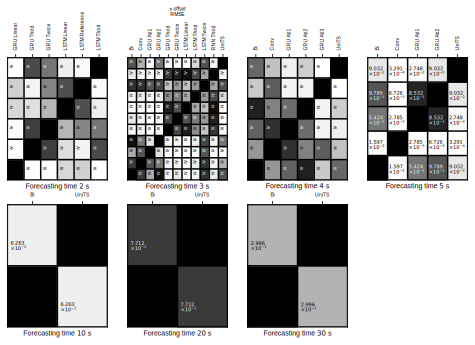
\includegraphics[width = 0.99 \linewidth]{var_long_RMSE.pdf}
	\caption{The $p$-values for the Wilcoxon signed-rank test on RMSE values across $k$-fold validation datasets for the $x$ offset in the $k$-fold testing datasets using different RNN models, and forecasting times. Darker colors in grayscale represent a higher $p$-value in a range from $0$ to $1$. The values on the secondary diagonal are all equal to $1$ and black because models equal themselves.}
	\label{fig:var_long_RMSE}
\end{figure}

The average RMSE in $\degree$ ($\times 10^{-4}$), with standard deviation in brackets, across $k$-fold validation datasets for the $x$ offset estimated on the $k$-fold testing datasets by different RNN models, and forecasting times is listed in Table~\ref{tab:wilcoxon_longitude_no_abs_RMSE}.

\begin{table}[!ht]
	\centering
	\resizebox{\linewidth}{!}{
		\begin{tabular}{|c|c|c|c|c|c|c|c|}
			\hline
			Model & $2$ $s$ & $3$ $s$ & $4$ $s$ & $5$ $s$ & $10$ $s$ & $20$ $s$ & $30$ $s$ \\ \hline
			\multirow{2}{*}{Bi} & $1.512$ & $1.903$ & $2.257$ & $2.589$ & $3.74$ & $4.936$ & $\mathbf{5.52}$ \\
			 & ($0.154$) & ($0.196$) & ($0.231$) & ($0.257$) & ($0.327$) & ($0.333$) & \textbf{(}$\mathbf{0.397}$\textbf{)} \\ \hline
			\multirow{2}{*}{Conv} & $1.447$ & $1.883$ & $2.521$ & $3.761$ & $5.564$ & $6.262$ & $6.376$ \\
			 & ($0.121$) & ($0.177$) & ($0.941$) & ($1.637$) & ($1.223$) & ($0.701$) & ($0.46$) \\ \hline
			\multirow{2}{*}{GRU Att 1} & $1.401$ & $\mathbf{1.846}$ & $2.265$ & $2.541$ & $4.544$ & $6.046$ & $6.47$ \\
			 & ($0.188$) & \textbf{(}$\mathbf{0.24}$\textbf{)} & ($0.271$) & ($0.274$) & ($0.694$) & ($0.471$) & ($0.597$) \\ \hline
			\multirow{2}{*}{GRU Att 2} & $1.44$ & $1.901$ & $2.256$ & $2.578$ & $3.85$ & $5.694$ & $6.756$ \\
			 & ($0.183$) & ($0.254$) & ($0.266$) & ($0.356$) & ($0.467$) & ($0.627$) & ($0.734$) \\ \hline
			\multirow{2}{*}{GRU Att 3} & $1.512$ & $1.973$ & $2.337$ & $2.72$ & $4.241$ & $6.355$ & $7.279$ \\
			 & ($0.178$) & ($0.247$) & ($0.272$) & ($0.286$) & ($0.614$) & ($0.823$) & ($1.112$) \\ \hline
			\multirow{2}{*}{GRU Linear} & $1.351$ & $2.063$ & $2.717$ & $3.068$ & $4.702$ & $6.637$ & $7.354$ \\
			 & ($0.2$) & ($0.25$) & ($0.353$) & ($0.319$) & ($0.399$) & ($0.461$) & ($0.46$) \\ \hline
			\multirow{2}{*}{GRU Third} & $1.134$ & $2.086$ & $2.758$ & $3.145$ & $4.76$ & $6.595$ & $7.331$ \\
			 & ($0.241$) & ($0.373$) & ($0.308$) & ($0.321$) & ($0.435$) & ($0.491$) & ($0.473$) \\ \hline
			\multirow{2}{*}{GRU Twice} & $1.207$ & $2.055$ & $2.641$ & $3.129$ & $4.737$ & $6.507$ & $7.293$ \\
			 & ($0.32$) & ($0.336$) & ($0.339$) & ($0.232$) & ($0.403$) & ($0.516$) & ($0.426$) \\ \hline
			\multirow{2}{*}{LSTM Linear} & $1.272$ & $2.083$ & $2.607$ & $3.142$ & $4.724$ & $6.601$ & $7.241$ \\
			 & ($0.29$) & ($0.303$) & ($0.292$) & ($0.266$) & ($0.386$) & ($0.53$) & ($0.449$) \\ \hline
			\multirow{2}{*}{LSTM Reference} & $1.256$ & $2.178$ & $2.732$ & $3.082$ & $4.701$ & $6.501$ & $7.308$ \\
			 & ($0.283$) & ($0.319$) & ($0.359$) & ($0.365$) & ($0.408$) & ($0.517$) & ($0.538$) \\ \hline
			\multirow{2}{*}{LSTM Third} & $\mathbf{1.123}$ & $2.014$ & $2.601$ & $3.145$ & $4.704$ & $6.568$ & $7.272$ \\
			 & \textbf{(}$\mathbf{0.201}$\textbf{)} & ($0.379$) & ($0.368$) & ($0.363$) & ($0.408$) & ($0.475$) & ($0.428$) \\ \hline
			\multirow{2}{*}{LSTM Twice} & $3.38$ & $2.326$ & $2.601$ & $3.046$ & $4.65$ & $6.51$ & $7.196$ \\
			 & ($2.409$) & ($1.522$) & ($0.542$) & ($0.407$) & ($0.401$) & ($0.458$) & ($0.457$) \\ \hline
			\multirow{2}{*}{RNN Third} & $1.758$ & $2.083$ & $2.767$ & $3.234$ & $4.713$ & $6.692$ & $7.376$ \\
			 & ($0.611$) & ($0.386$) & ($0.427$) & ($0.419$) & ($0.374$) & ($0.565$) & ($0.497$) \\ \hline
			\multirow{2}{*}{UniTS} & $1.582$ & $1.917$ & $\mathbf{2.219}$ & $\mathbf{2.494}$ & $\mathbf{3.565}$ & $\mathbf{4.895}$ & $5.654$ \\
			 & ($0.178$) & ($0.202$) & \textbf{(}$\mathbf{0.224}$\textbf{)} & \textbf{(}$\mathbf{0.244}$\textbf{)} & \textbf{(}$\mathbf{0.319}$\textbf{)} & \textbf{(}$\mathbf{0.404}$\textbf{)} & ($0.433$) \\ \hline
		\end{tabular}
	}
	\caption{The average RMSE in $\degree$ ($\times 10^{-4}$), with standard deviation in brackets, across $k$-fold validation datasets for the $x$ offset estimated on the $k$-fold testing datasets by different RNN models, and forecasting times.}
	\label{tab:wilcoxon_longitude_no_abs_RMSE}
\end{table}

The Bi model achieved the lowest RMSE for $x$ offset, and a forecasting time of $30$ $s$ with an average value and standard deviation (in brackets) that equals $5.52 \times 10^{-4}$ $\degree$ ($0.397 \times 10^{-4}$ $\degree$).

The Bi model does not have a statistically significantly different RMSE than the UniTS model for $x$ offset using a forecasting time of $30$ $s$, with a $p$-value equaling $2.996 \times 10^{-1}$.

\markertable{tab:\label{tab:RMSE:longitude:no:abs:p:30}}

The GRU Att 1 model achieved the lowest RMSE for $x$ offset, and a forecasting time of $3$ $s$ with an average value and standard deviation (in brackets) that equals $1.846 \times 10^{-4}$ $\degree$ ($0.24 \times 10^{-4}$ $\degree$).

The GRU Att 1 model does not have a statistically significantly different RMSE than the Bi, Conv, GRU Att 2, GRU Third, GRU Twice, LSTM Linear, LSTM Third, LSTM Twice, RNN Third, and UniTS models for $x$ offset using a forecasting time of $3$ $s$, with $p$-values equaling $3.254 \times 10^{-1}$, $6.721 \times 10^{-1}$, $1.073 \times 10^{-1}$, $2.255 \times 10^{-3}$, $4.605 \times 10^{-3}$, $5.564 \times 10^{-4}$, $2.027 \times 10^{-2}$, $9.789 \times 10^{-1}$, $3.764 \times 10^{-4}$, and $7.15 \times 10^{-4}$.

\markertable{tab:\label{tab:RMSE:longitude:no:abs:p:3}}

The LSTM Third model achieved the lowest RMSE for $x$ offset, and a forecasting time of $2$ $s$ with an average value and standard deviation (in brackets) that equals $1.123 \times 10^{-4}$ $\degree$ ($0.201 \times 10^{-4}$ $\degree$).

The LSTM Third model does not have a statistically significantly different RMSE than the GRU Linear, GRU Third, GRU Twice, LSTM Linear, and LSTM Reference models for $x$ offset using a forecasting time of $2$ $s$, with $p$-values equaling $6.313 \times 10^{-4}$, $7.112 \times 10^{-1}$, $5.424 \times 10^{-1}$, $6.263 \times 10^{-2}$, and $2.027 \times 10^{-2}$.

\markertable{tab:\label{tab:RMSE:longitude:no:abs:p:2}}

The UniTS model achieved the lowest RMSE for $x$ offset, and a forecasting time of $4$, $5$, $10$, and $20$ $s$ with average values and standard deviation (in brackets) that equal $2.219 \times 10^{-4}$ $\degree$ ($0.224 \times 10^{-4}$ $\degree$), $2.494 \times 10^{-4}$ $\degree$ ($0.244 \times 10^{-4}$ $\degree$), $3.565 \times 10^{-4}$ $\degree$ ($0.319 \times 10^{-4}$ $\degree$), and $4.895 \times 10^{-4}$ $\degree$ ($0.404 \times 10^{-4}$ $\degree$) respectively.

The UniTS model does not have a statistically significantly different RMSE than the Bi, Conv, GRU Att 1, GRU Att 2, and GRU Att 3 models for $x$ offset using a forecasting time of $4$ $s$, with $p$-values equaling $5.965 \times 10^{-1}$, $2.411 \times 10^{-1}$, $5.875 \times 10^{-2}$, $1.908 \times 10^{-1}$, and $3.291 \times 10^{-4}$.

\markertable{tab:\label{tab:RMSE:longitude:no:abs:p:4}}

The UniTS model does not have a statistically significantly different RMSE than the Bi, Conv, GRU Att 1, and GRU Att 2 models for $x$ offset using a forecasting time of $5$ $s$, with $p$-values equaling $9.032 \times 10^{-2}$, $3.291 \times 10^{-4}$, $2.748 \times 10^{-2}$, and $9.032 \times 10^{-2}$.

\markertable{tab:\label{tab:RMSE:longitude:no:abs:p:5}}

The UniTS model does not have a statistically significantly different RMSE than the Bi model for $x$ offset using a forecasting time of $10$ $s$, with a $p$-value equaling $6.263 \times 10^{-2}$.

\markertable{tab:\label{tab:RMSE:longitude:no:abs:p:10}}

The UniTS model does not have a statistically significantly different RMSE than the Bi model for $x$ offset using a forecasting time of $20$ $s$, with a $p$-value equaling $7.712 \times 10^{-1}$.

\markertable{tab:\label{tab:RMSE:longitude:no:abs:p:20}}

